\chapter{Capitolo 1: Concetti base di biologia}
La bioinformatica è una materia che tratta tanto l'informatica quanto la biologia, pertanto è necessario illustrarne gli argomenti più importanti, che verranno spiegati in modo funzionale allo scopo della presente tesi.
\newline
La \textit{biologia} è la scienza che studia la vita, dagli attori che ne fanno parte fino ai processi in cui essi sono coinvolti \cite{campbellBiology}. Poiché la vita nella terra si estende dalle molecole fino alla biosfera, si è resa necessaria l'esigenza di trovare una vera e propria scala a livello globale. Tra le varie forme di vita si trovano, omettendo quelle non interessate ed in ordine crescente, le molecole (insiemi di atomi), le macromolecole (insieme di molecole) e le cellule (insieme di macromolecole).
\newline
Ci sono quattro tipi di macromolecole che risultano essenziali per tutte le forme di vita:
\begin{itemize}
	\item \textit{Polisaccaridi}: macromolecole formate da un'insieme molecole di monosaccaridi, tra cui il fruttosio, il glucosio e così via.
	\item \textit{Proteine}: sono la "struttura" degli esseri viventi, consentendo lo sviluppo e mantenimento degli organi.
	\item \textit{Lipidi}: chiamati anche grassi, sono le riserve di energia.
	\item \textit{Acidi nucleici}: DNA e RNA.
\end{itemize}
Di seguito vengono approfonditi il DNA, l'RNA e le proteine.
\newpage

\section{DNA}
Il \textit{DNA} o \textit{acido desossiribonucleico} è una macromolecola contenente il patrimonio genetico\footnote{Il patrimonio genetico contiene tutte le informazioni genetiche di un organismo.} degli esseri viventi \cite{campbellBiology}, pertanto ne detiene l'informazione ereditaria \cite{BiologySolomon}.
\newline
Di seguito viene illustrata un'immagine del DNA, insieme ad una breve descrizione.
\newline
\begin{figure}[h!]
	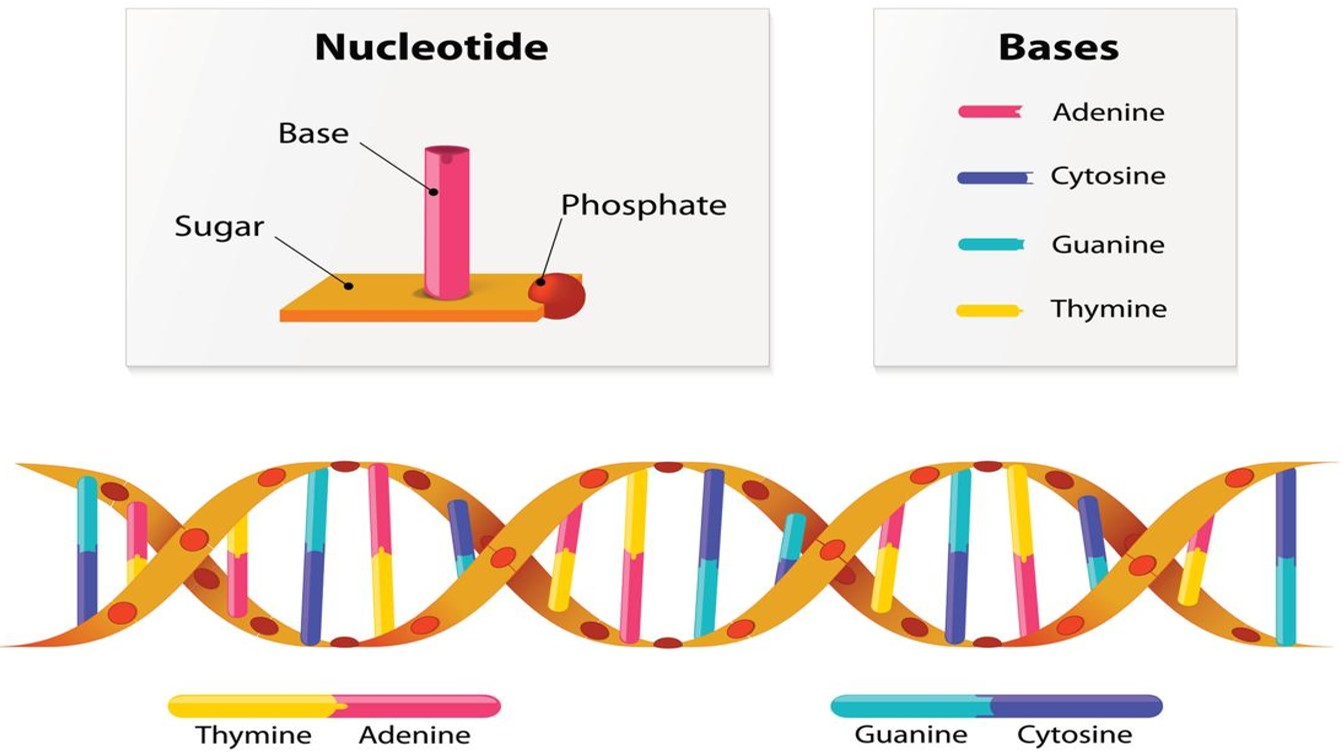
\includegraphics[width=\linewidth]{DNAStructure.jpg}
 	\caption{La struttura del DNA e del nucleotide.}
  	\label{fig:DnaAndNucleotideStructure}
\end{figure}
\newline
La struttura è caratterizzata da una doppia elica, dove ciascun filamento è formato da una sequenza di molecole di lunghezza variabile chiamate \textit{nucleotidi}.
\newline
Un nucleotide è composto da una molecola di zucchero, un gruppo fosfato\footnote{Il gruppo fosfato è un un insieme di elementi strutturati e ben definiti.} ed una base azotata. Di quest'ultima, ne esistono quattro tipi:
\begin{itemize}
	\item \textit{adenina} (A);
	\item \textit{timina} (T);
	\item \textit{guanina} (G);
	\item \textit{citosina} (C).
\end{itemize}
Una proprietà importante delle basi azotate è che l'Adenina si può legare solo la Timina (A-T), mentre la Guanina con la Citosina (G-C). Questo significa che i filamenti sono complementari e quindi se conosciamo le basi di un filamento sappiamo pure quelle dell'altro.

\section{RNA}
L'\textit{RNA}, ovvero \textit{acido ribonucleico}, è una macromolecola caratterizzata da una struttura a singolo filamento composta da una \textit{sequenza di ribonucleotidi} di lunghezza variabile.
\newline
I ribonucleotidi si differenziano rispetto ai nucleotidi per una diversa molecola di zucchero e per la Timina (T) che è sostituita con l'Uracile (U).
\newline
Un tipo di RNA importante per la sintesi delle proteine è l'\textit{RNA messaggero} (mRNA), che trasporta l'informazione genetica contenuta nel DNA nella zona della cellula in cui avviene la sintesi delle proteine\footnote{La sintesi proteica è il processo attraverso il quale vengono prodotte nuove proteine.}.

\section{Proteine}
Le proteine sono le fondamenta di un organismo, infatti determinano la struttura e le funzioni delle cellule, ad esempio le cellule del cervello differiscono da quelle dei muscoli principalmente perché usano tipi di proteine diverse.
La loro struttura è composta da sequenze di \textit{aminoacidi} legati tra loro. Sebbene ne esistano oltre cinquecento in natura, ne vengono usati solo venti per la sintesi proteica.